\section{Results}
\subsection{Analysis for t\textless0}
\label{ssec:lessthan}
The solution of the matrix and the respective table with the nodal analysis results from section ~\ref{ssec:tl}, obtained using \textit{octave}, can be seen below.\\
$ \left(\begin{array}{c} V_1 \\ V_2 \\ V_3 \\ V_5 \\ V_6 \\ V_7 \\ V_8 \end{array}\right)= \left(\begin{array}{c} 5.233347 \\ 4.993818 \\ 4.495480 \\ 5.028594 \\ 5.796288 \\ -2.004014 \\ -3.034274 \end{array}\right) $
 \begin{table}[H]
 \footnotesize
 \centering
 \caption{Nodal Analysis results for t<0}
 \label{tab:tables}
 \begin{center}
 \begin{tabular}{cccc}
\hline 
 Node & Voltage (V) & R & Current(mA) \\ 
 \hline 
 1 & 5.233347& $R_1$ & -0.233449 \\ 
 \hline 
 2& 4.993818 & $R_2$ & -0.244673\\ 
 \hline 
 3 & 4.495480& $R_3$ & -0.011224 \\ 
 \hline 
 4 & 0 &$R_4$ & 1.225637 \\ 
 \hline 
 5 &5.028594& $R_5$ & 0.244673\\ 
 \hline 
 6 & 5.796288 & $R_6$ & -0.992188\\ 
 \hline 
 7 & -2.004014 & $R_7$ & -0.992188\\ 
 \hline 
 8 & -3.034274 & $I_b$ & -0.244673 \\ 
 \hline \end{tabular} 
 \end{center} 
 \end{table}
The respective ngspice simulation results, to compare with the previous ones can be seen in Table 2.\\
\begin{table}[H]
  \centering
  \begin{tabular}{|l|r|}
    \hline    
    {\bf Name} & {\bf Value [A or V]} \\ \hline
    @g1[i] & -2.44673e-04\\ \hline
@i1[current] & 1.046207e-03\\ \hline
@r1[i] & 2.334490e-04\\ \hline
@r2[i] & 2.446726e-04\\ \hline
@r3[i] & -1.12237e-05\\ \hline
@r4[i] & -1.22564e-03\\ \hline
@r5[i] & -1.29088e-03\\ \hline
@r6[i] & 9.921880e-04\\ \hline
@r7[i] & 9.921880e-04\\ \hline
v(1) & 5.233347e+00\\ \hline
v(2) & 4.993818e+00\\ \hline
v(3) & 4.495481e+00\\ \hline
v(4) & 5.028594e+00\\ \hline
v(5) & 9.078902e+00\\ \hline
v(6) & -2.00401e+00\\ \hline
v(7) & -2.00401e+00\\ \hline
v(8) & -3.03427e+00\\ \hline

  \end{tabular}
  \caption{Operating point. A variable preceded by @ is of type {\em current}
    and expressed in Ampere; other variables are of type {\it voltage} and expressed in
    Volt.}
  \label{tab:op}
\end{table}

\subsection{Analysis for t=0}
\label{ssec:equal}
The solution of the matrix and the respective table with the nodal analysis results from section ~\ref{ssec:R}, obtained using \textit{octave}, can be seen below.Here we also get $I_x$ and $R_{eq}$.\\
$ \left(\begin{array}{c} V_1 \\ V_2 \\ V_3 \\ V_5 \\ V_6 \\ V_7 \\ V_8 \end{array}\right)= \left(\begin{array}{c} 0.000000 \\ 0.000000 \\ 0.000000 \\ 0.000000 \\ 8.830562 \\ 0.000000 \\ 0.000000 \end{array}\right) $
 \begin{table}[H]
 \footnotesize
 \centering
 \caption{Nodal Analysis results}
 \label{tab:tables}
 \begin{center}
 \begin{tabular}{cccc}
\hline 
 Node & Voltage (V) & R & Current(mA) \\ 
 \hline 
 1 & 0.000000& $R_1$ & 0.000000 \\ 
 \hline 
 2& 0.000000 & $R_2$ & 0.000000\\ 
 \hline 
 3 & 0.000000& $R_3$ & 0.000000 \\ 
 \hline 
 4 & 0 &$R_4$ & 0.000000 \\ 
 \hline 
5 &0.000000& $R_5$ & 2.814401\\ 
 \hline 
 6 & 8.830562 & $R_6$ & 0.000000\\ 
 \hline 
 7 & 0.000000 & $R_7$ & 0.000000\\ 
 \hline 
 8 & 0.000000 & $I_b$ & 0.000000 \\ 
 \hline 
 \end{tabular} 
 \end{center} 
 \end{table}
 $Ix=-2.814401 mA$  $Req=3.137634 k\Omega$ $\tau=0.003283$
The same analysis using ngspice yields the following results.\\
\begin{table}[H]
  \centering
  \begin{tabular}{|l|r|}
    \hline    
    {\bf Name} & {\bf Value [A or V]} \\ \hline
    @g1[i] & -2.12269e-18\\ \hline
@r1[i] & 2.025320e-18\\ \hline
@r2[i] & 2.122693e-18\\ \hline
@r3[i] & -9.73728e-20\\ \hline
@r4[i] & 4.329577e-19\\ \hline
@r5[i] & 2.814401e-03\\ \hline
@r6[i] & -4.33681e-19\\ \hline
@r7[i] & -8.67138e-19\\ \hline
v(1) & 0.000000e+00\\ \hline
v(2) & -2.07807e-15\\ \hline
v(3) & -6.40146e-15\\ \hline
v(5) & -1.77636e-15\\ \hline
v(6) & 8.830562e+00\\ \hline
v(7) & 8.759452e-16\\ \hline
v(8) & 1.776357e-15\\ \hline
v(9) & 8.759452e-16\\ \hline

  \end{tabular}
  \caption{Operating point. A variable preceded by @ is of type {\em current}
    and expressed in Ampere; other variables are of type {\it voltage} and expressed in
    Volt.}
  \label{tab:ops}
\end{table}
Here we also got, for Ix\footnote{using 96514 as the generating number}, -2.81440 mA.\\
\subsection{t\textgreater0: Natural Response}
The plot for the natural of the voltage in node 6, as a function of time can be seen in Figure ~\ref{fig:rc1}.\\
\begin{figure}[H] \centering
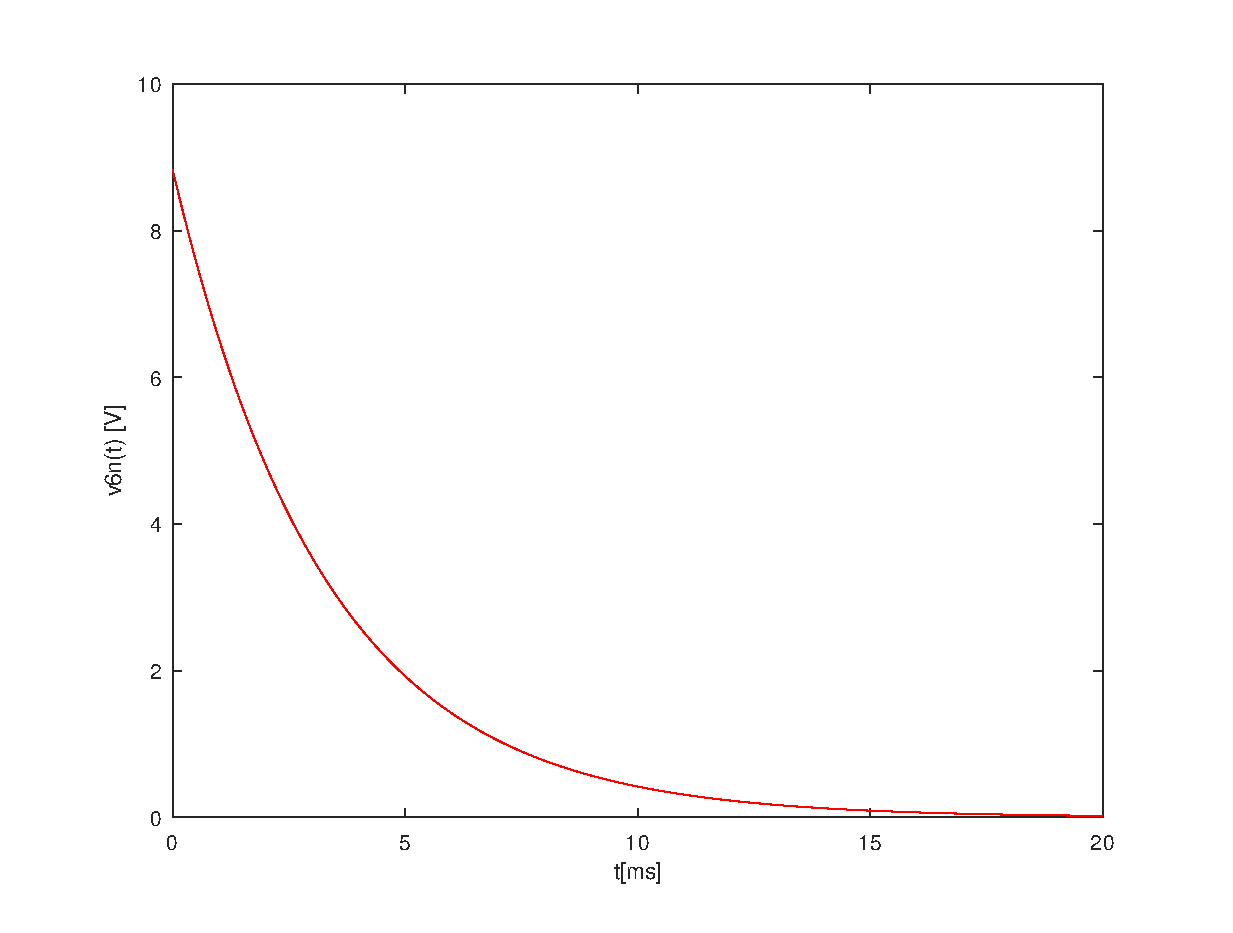
\includegraphics[width=0.4\linewidth]{natural.eps}
\caption{Natural response of V6 [0,20]ms using octave}
\label{fig:rc1}
\end{figure}

The same plot, obtained by transient analysis using \textit{ngspice}, is in Figure ~\ref{fig:rc2}.\\
\begin{figure}[H] \centering
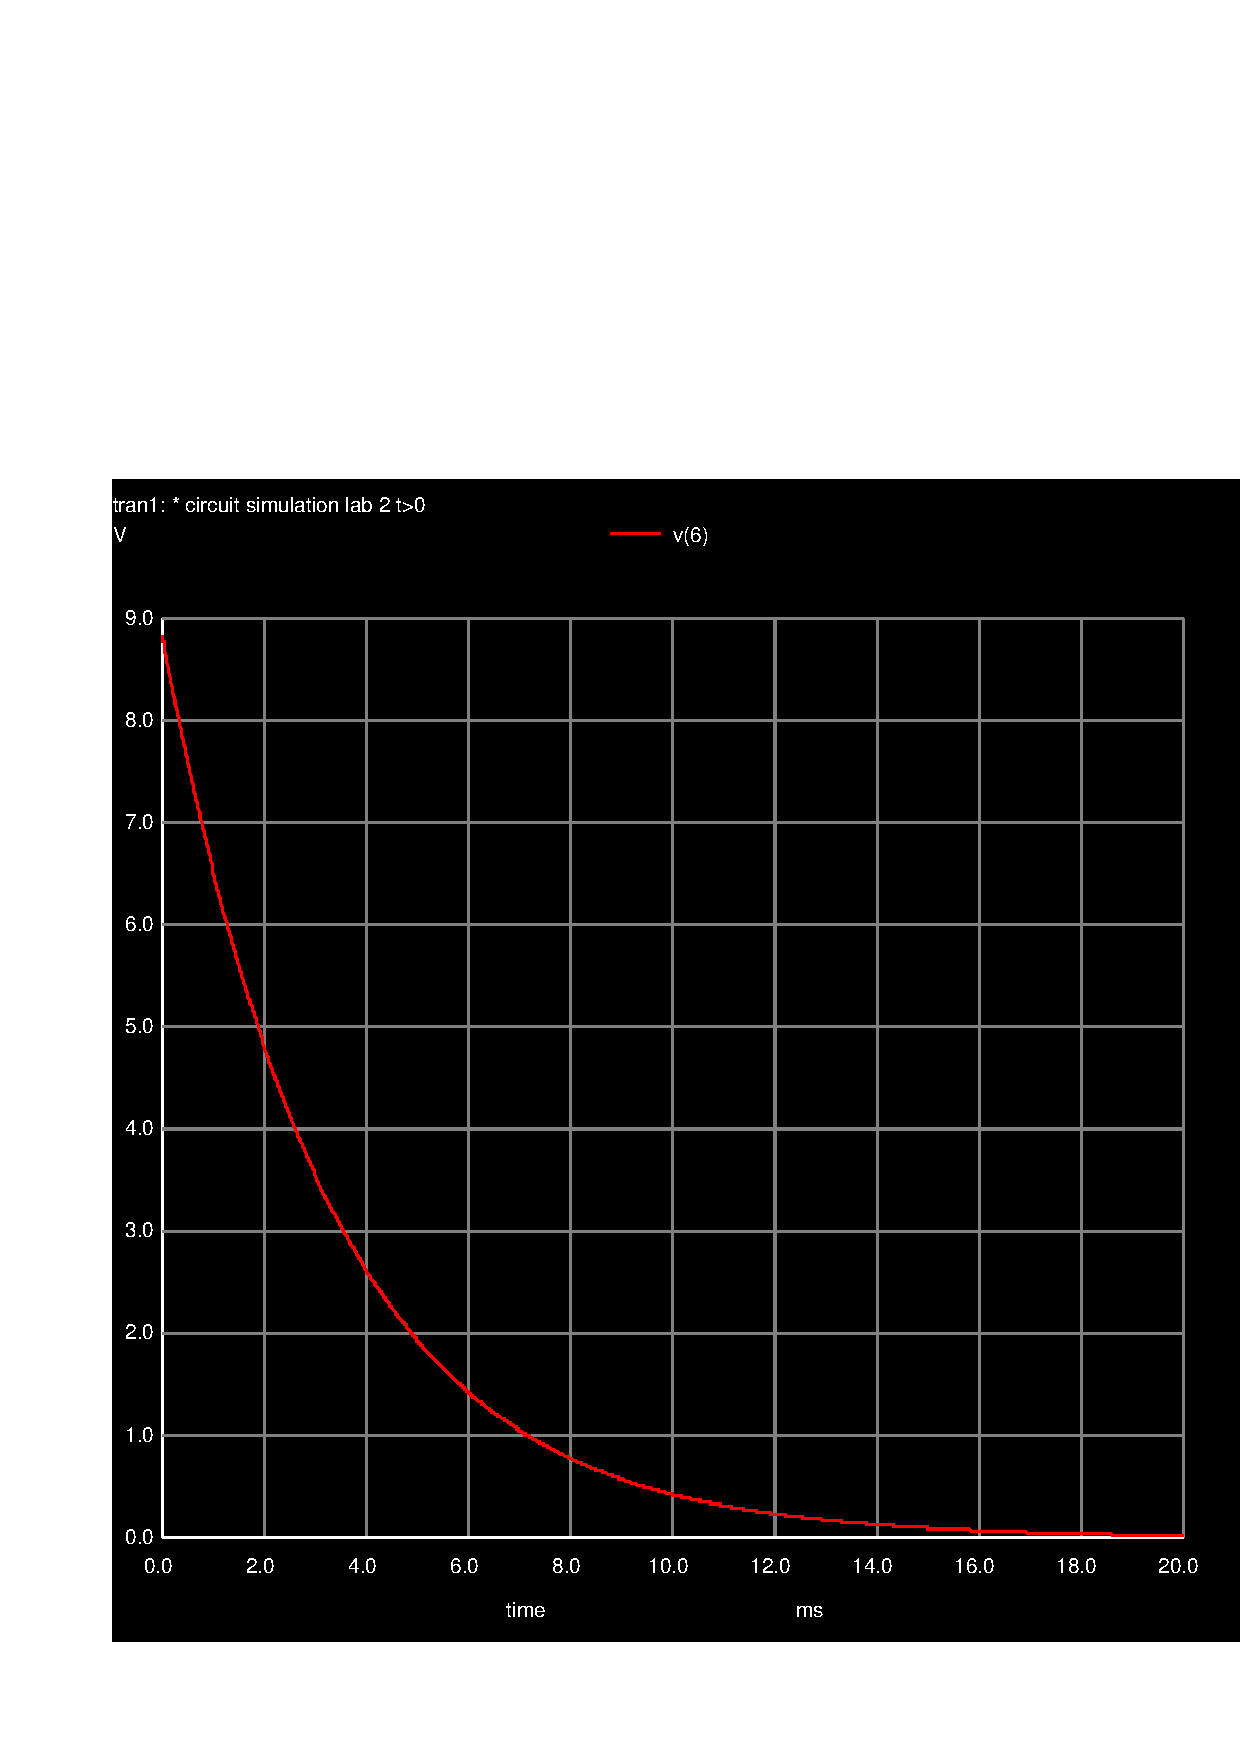
\includegraphics[width=0.4\linewidth]{../sim/trans.pdf}
\caption{Natural response of V6 in [0,20]ms using ngspice}
\label{fig:rc2}
\end{figure}
As we can see, we get the same result using both methods.

\subsection{t\textgreater0: Forced Response}
The phasor nodal voltages obtained can be seen in the table below.\\
$ \left(\begin{array}{c} V_1 \\ V_2 \\ V_3 \\ V_5 \\ V_6 \\ V_7 \\ V_8 \end{array}\right)= \left(\begin{array}{c} 5.233347 \\ 0.954230 \\ 0.859007 \\ 0.960875 \\ -0.579796 + -0.000082 i \\ -0.382932 \\ -0.579796 \end{array}\right) $
 \begin{table}[H]
 \footnotesize
 \centering
 \caption{Nodal Analysis results for t\textgreater0}
 \label{tab:tables}
 \begin{center}
 \begin{tabular}{ccc} 
 & Voltage (V)\\ 
 \hline 


 \hline 
 1 & 5.233347 \\ 
 \hline 
 2 & 0.954230 \\ 
 \hline 
 3 & 0.859007 \\ 
 \hline 
 4 & 0 \\ 
 \hline 
 5 & 0.960875 \\ 
 \hline 
 6 & -0.579796 + -0.000082 i \\ 
 \hline 
 7 & -0.382932 \\ 
 \hline 
 8 &  -0.579796 \\ 
 \hline 
 \\ 
  \end{tabular} 
 \end{center} 
 \end{table}
The plot of the forced component of V6 can be seen in Figure ~\ref{fig:ii}
 \begin{figure}[H] \centering
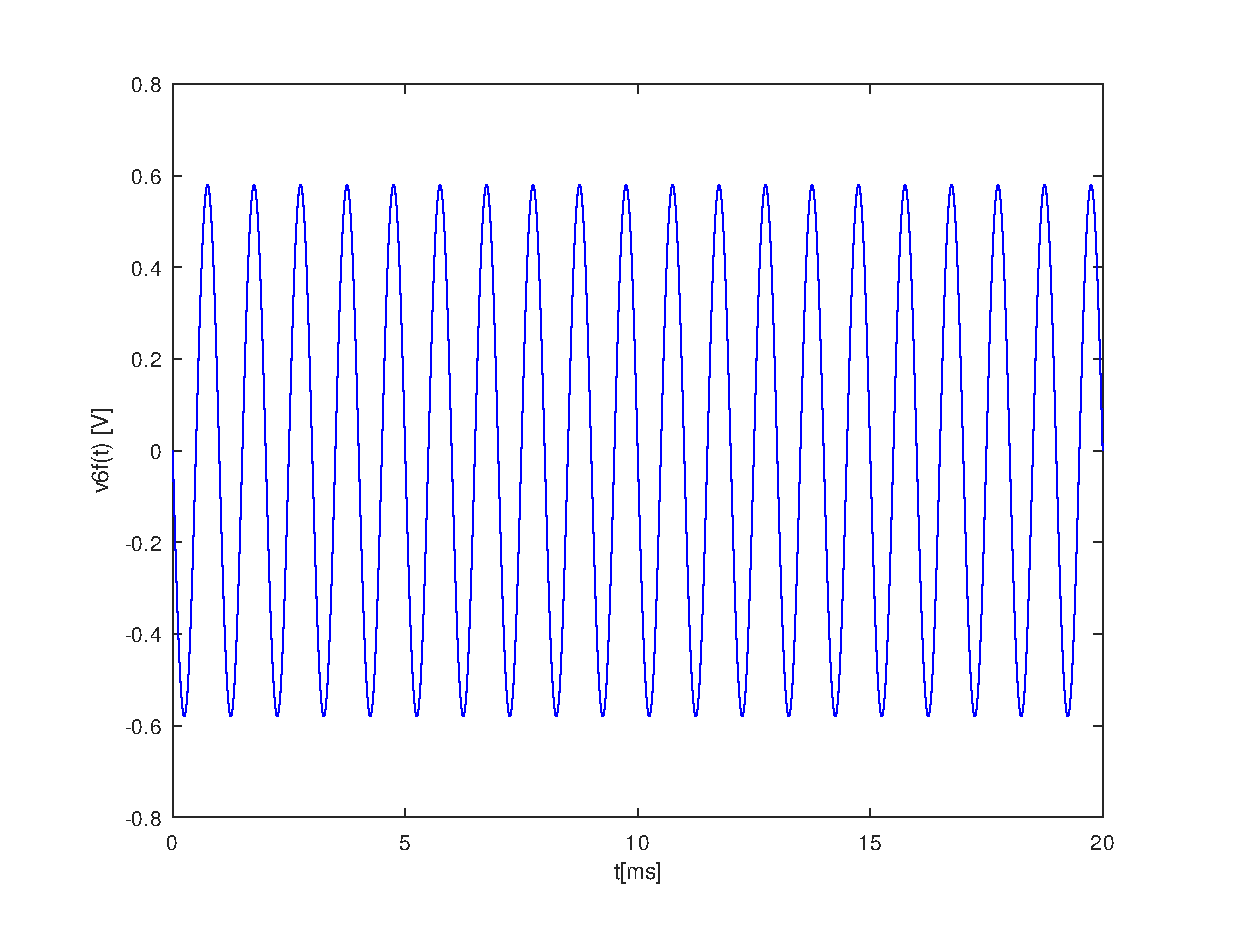
\includegraphics[width=0.4\linewidth]{forced.eps}
\caption{Force component of V6 in [0,20]ms using octave}
\label{fig:ii}
 \end{figure}

\subsection{t\textgreater0: Total Response}
  The plot of the full response of node 6 (with contributions from the natural and forced components) and the voltage in node 1, in the time interval [-5,20]ms, from \textit{octave} is in Figure ~\ref{fig:aa}.\\
 \begin{figure}[H] \centering
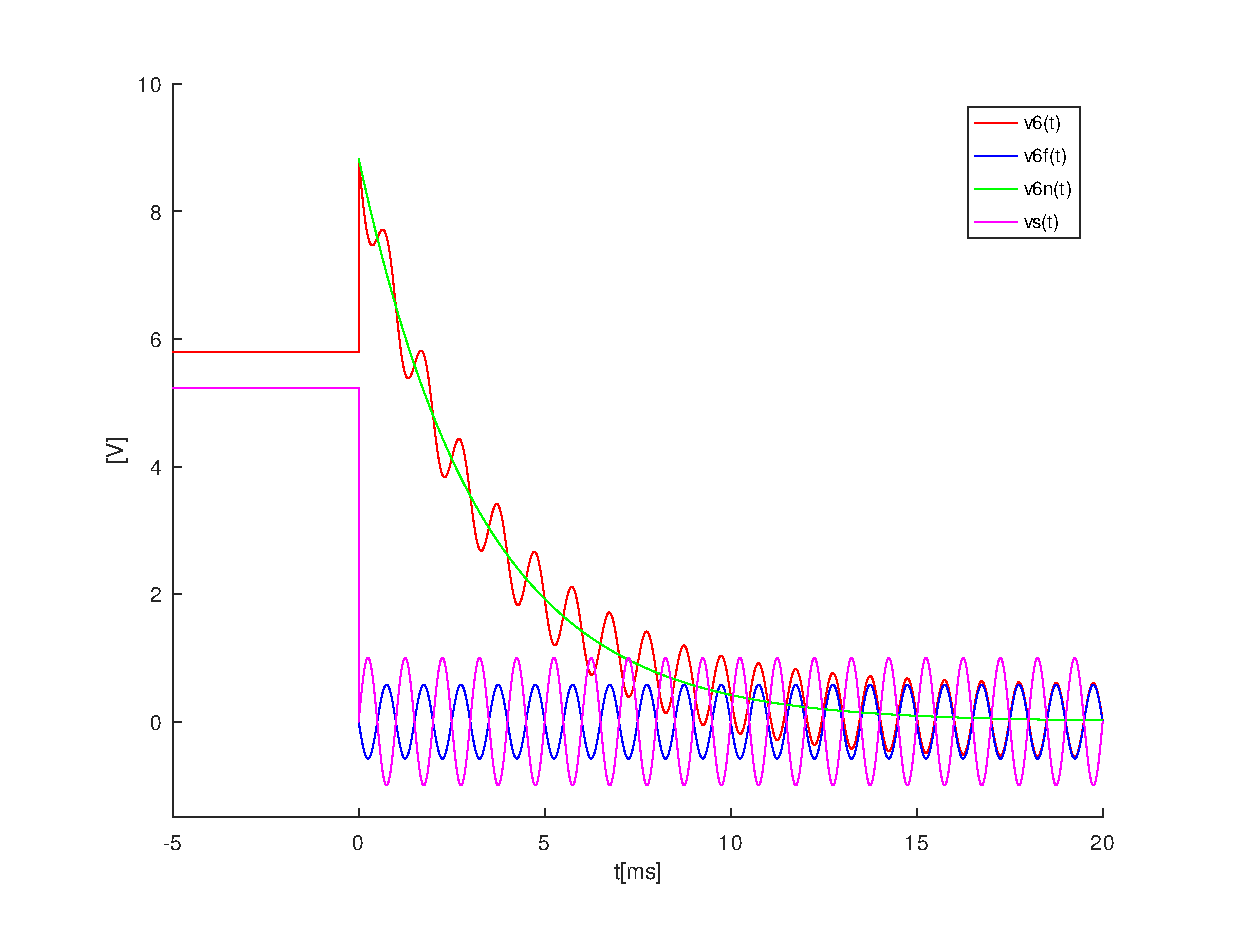
\includegraphics[width=0.4\linewidth]{total.eps}
\caption{V6 and V1 in [-5,20]ms  using octave}
\label{fig:aa}
 \end{figure}
 The same plot using ngpice in the time interval [0,20]ms, is in Figure ~\ref{fig:bb}
 \begin{figure}[H] \centering
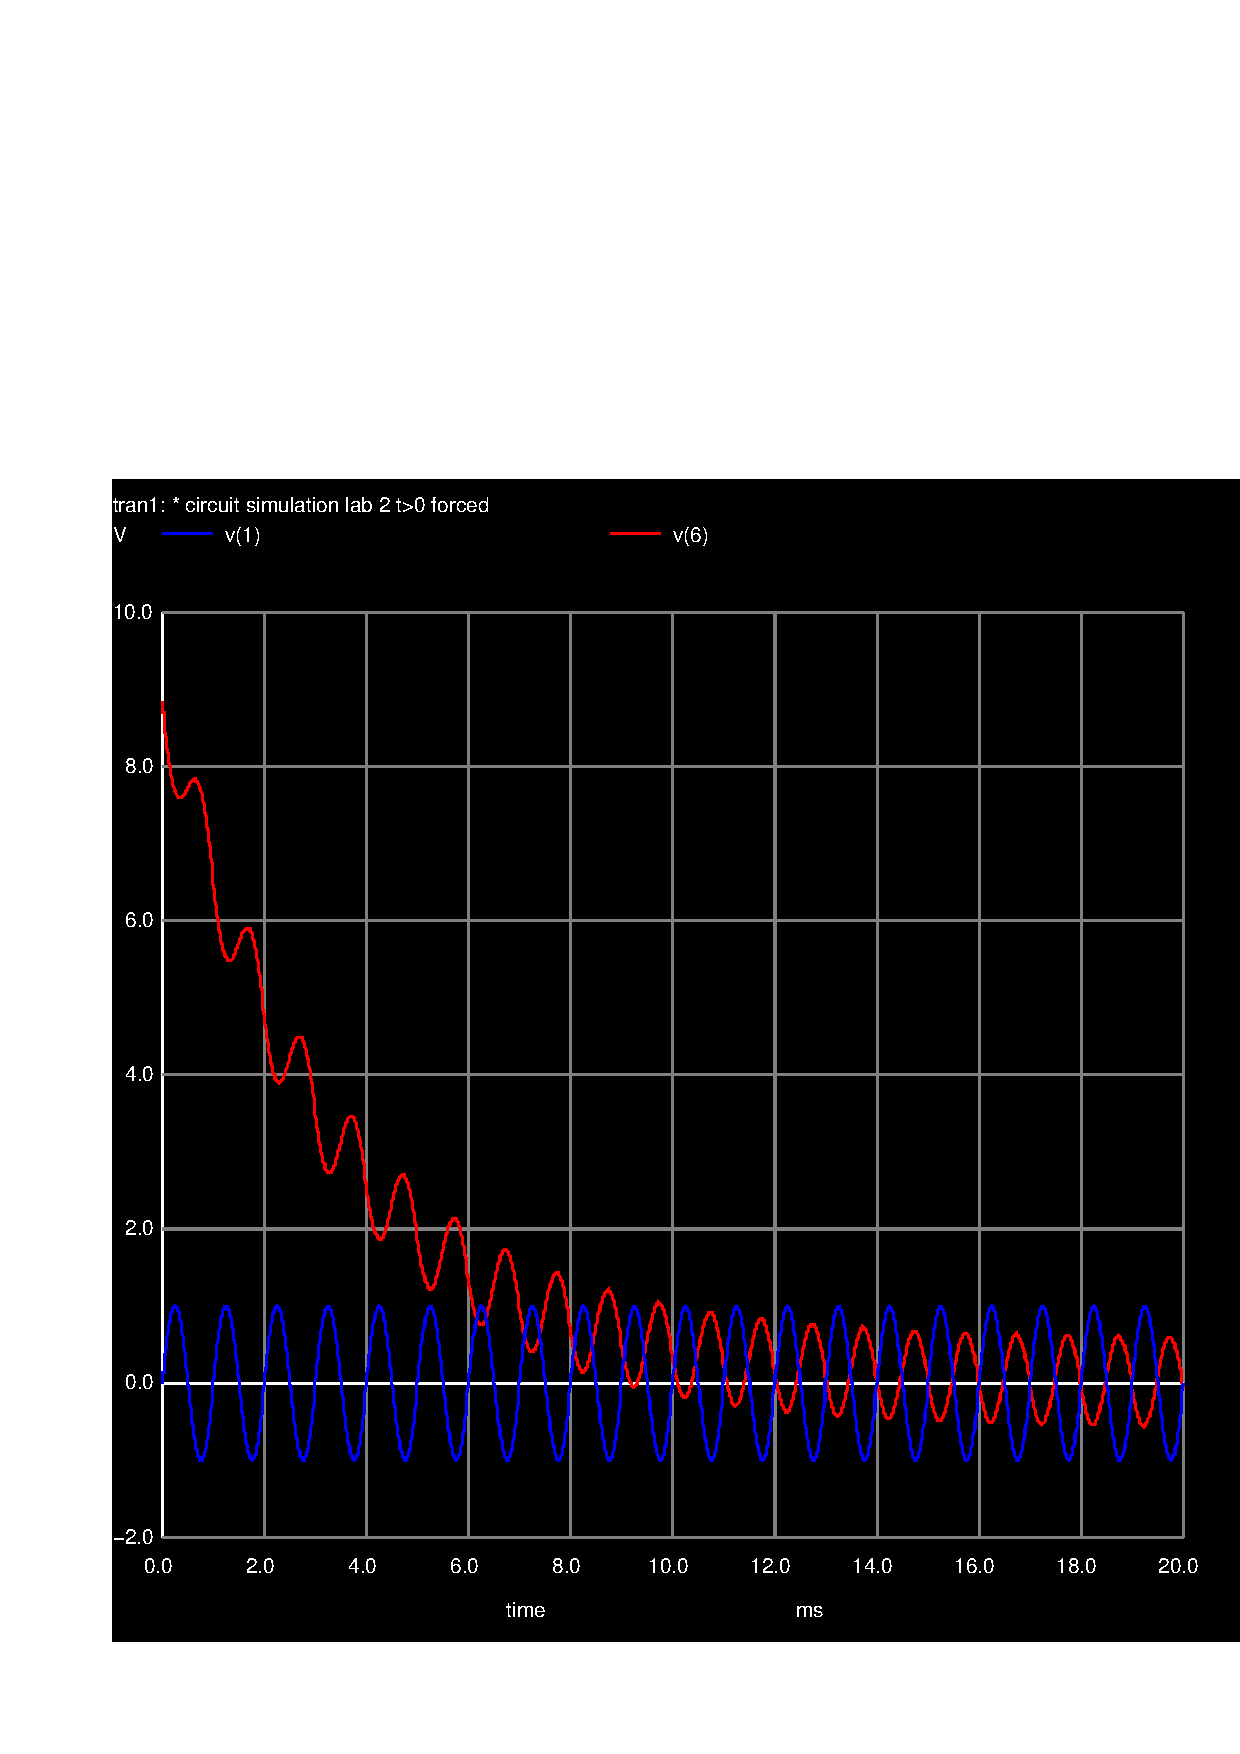
\includegraphics[width=0.4\linewidth]{../sim/tot.pdf}
\caption{V6 and V1 in [0,20]ms using ngspice}
\label{fig:bb}
\end{figure}

As we can see, we get the same results from both analysis.

\subsection{Frequency Analysis}
The plots of magnitude from frequency response in nodes 1 and 6, and in the capacitor, using \textit{octave} can be seen in Figure ~\ref{fig:cc}, and using \textit{ngspice} in Figure ~\ref{fig:dd}\\
 \begin{figure}[H] \centering
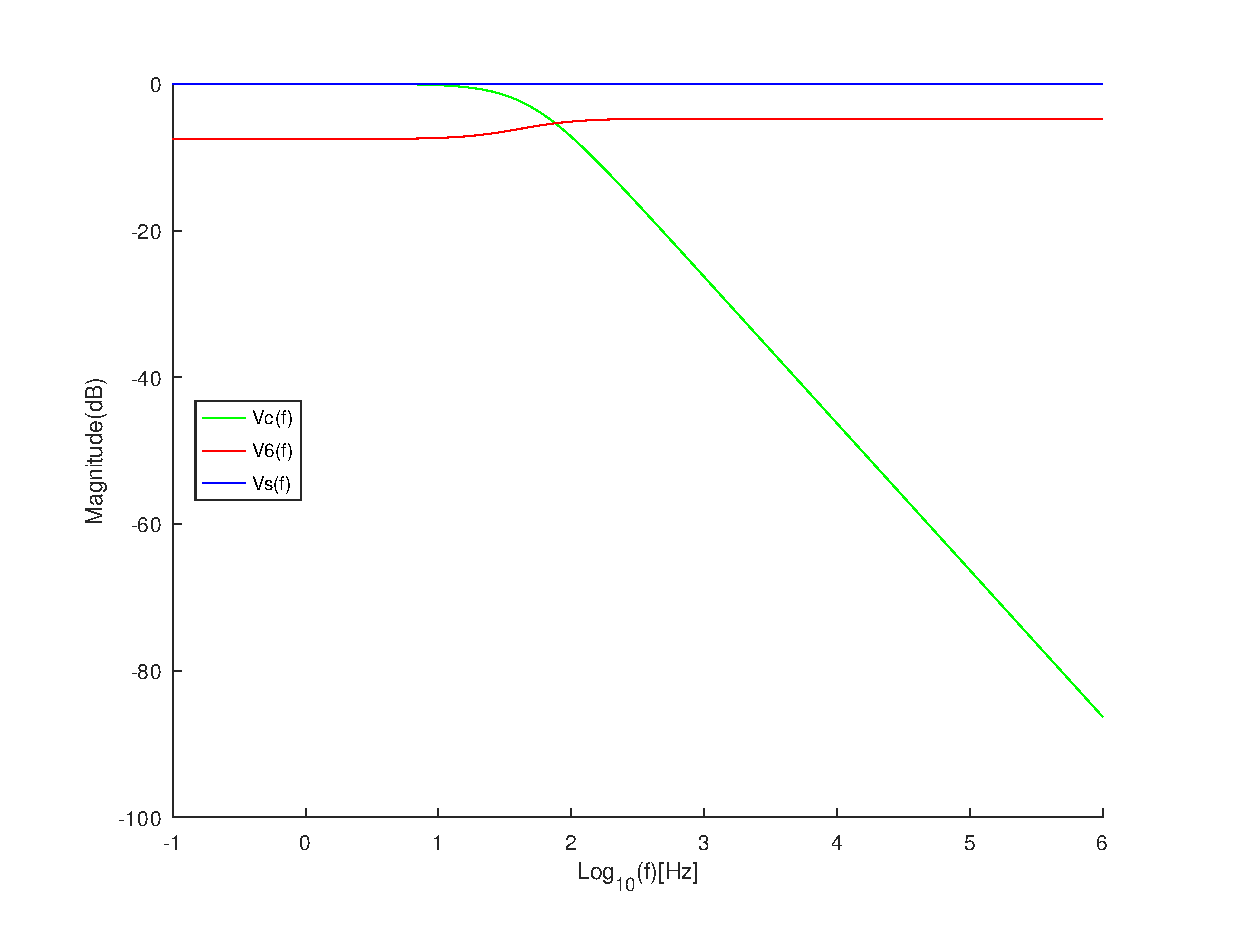
\includegraphics[width=0.4\linewidth]{Magnitude.eps}
\caption{Magnitude of V6(f),V1(f) and Vc(f) using octave}
\label{fig:cc}
 \end{figure}

  \begin{figure}[H] \centering
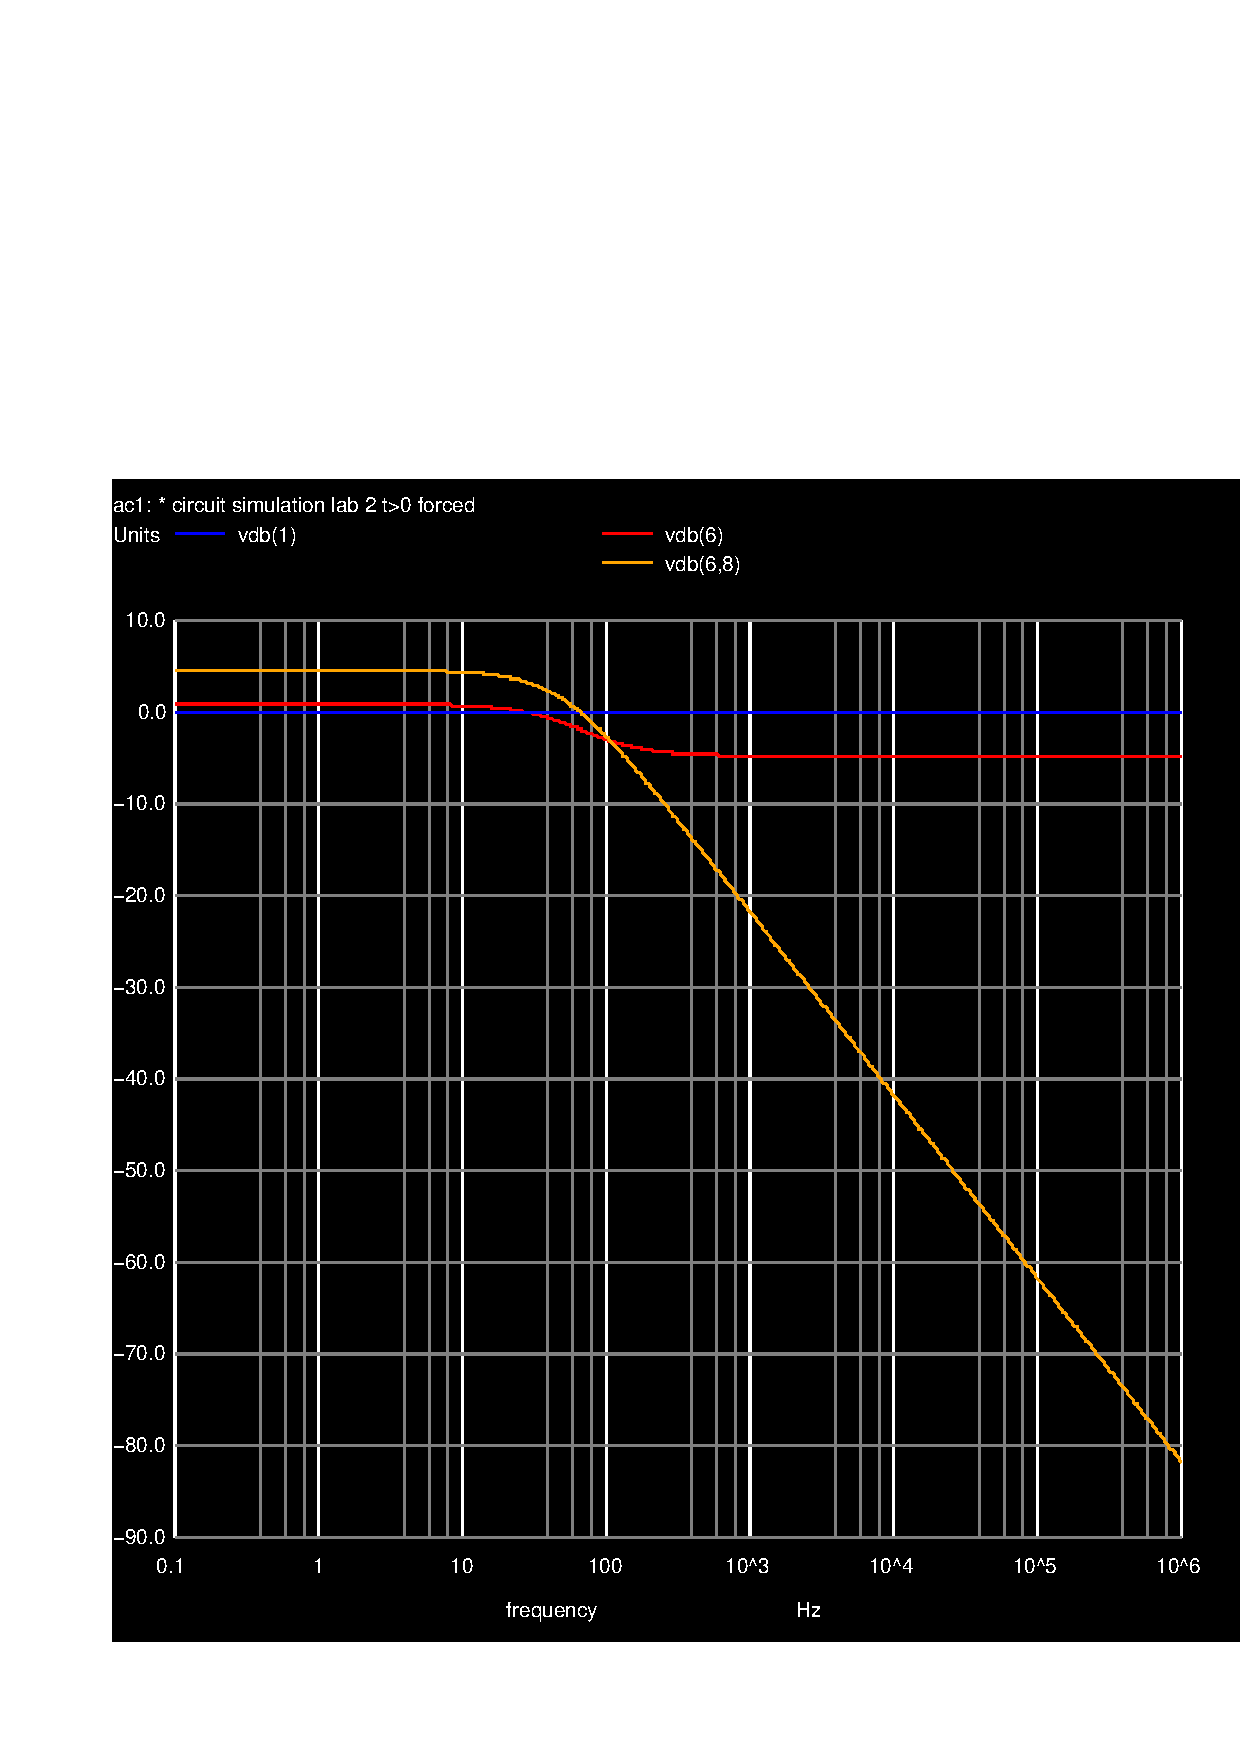
\includegraphics[width=0.4\linewidth]{../sim/mag.pdf}
\caption{Magnitude of V6(f),V1(f) and Vc(f) using ngspice}
\label{fig:dd}
\end{figure}

The plots of phase from frequency response in nodes 1 and 6, and in the capacitor, using \textit{octave} can be seen in Figure ~\ref{fig:ee}, and using \textit{ngspice} in Figure ~\ref{fig:ff}
 \begin{figure}[H] \centering
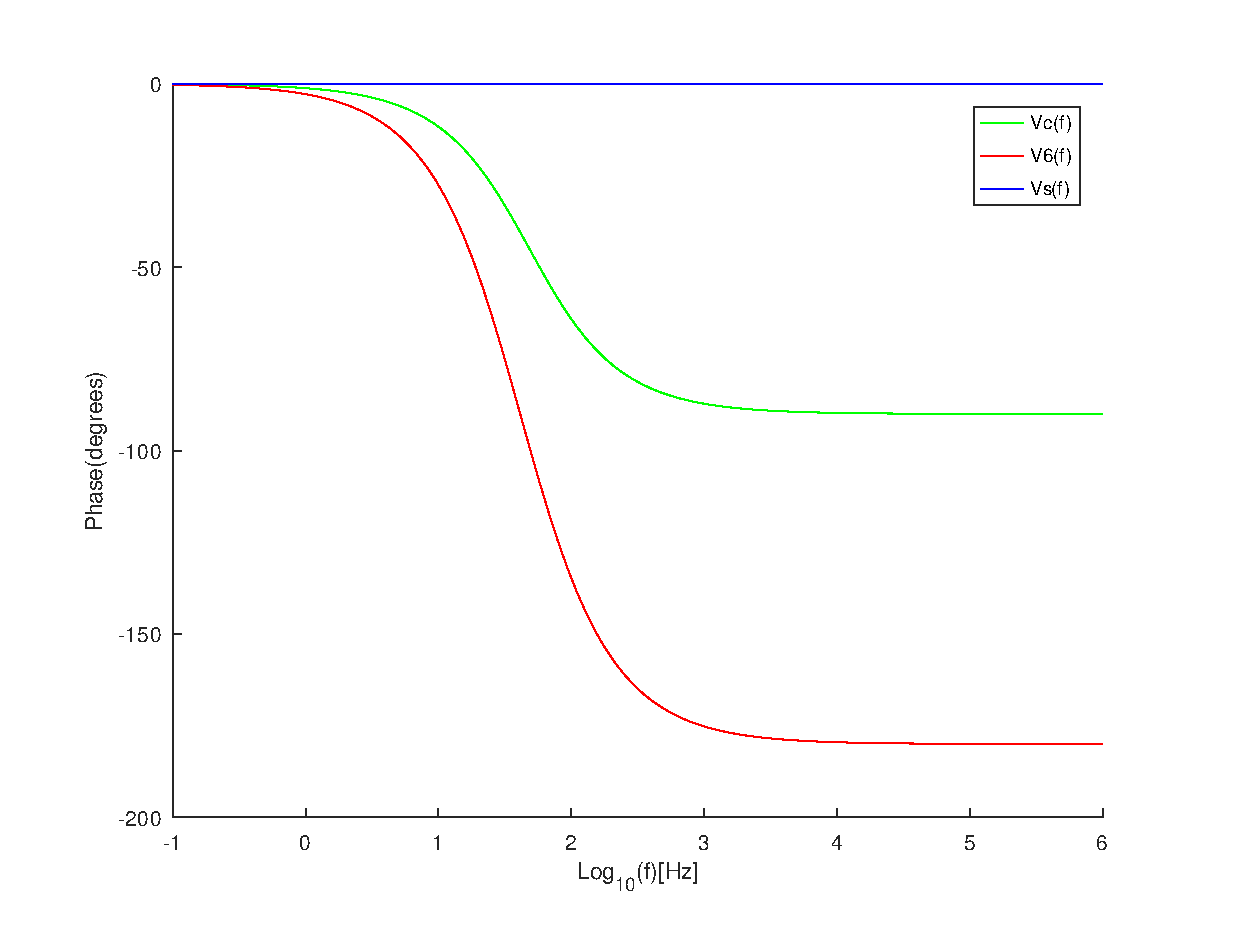
\includegraphics[width=0.4\linewidth]{Phase.eps}
\caption{Phase of V6(f), V1(f) and Vc(f) in [0,20]ms using octave}
\label{fig:ee}
 \end{figure}

  \begin{figure}[H] \centering
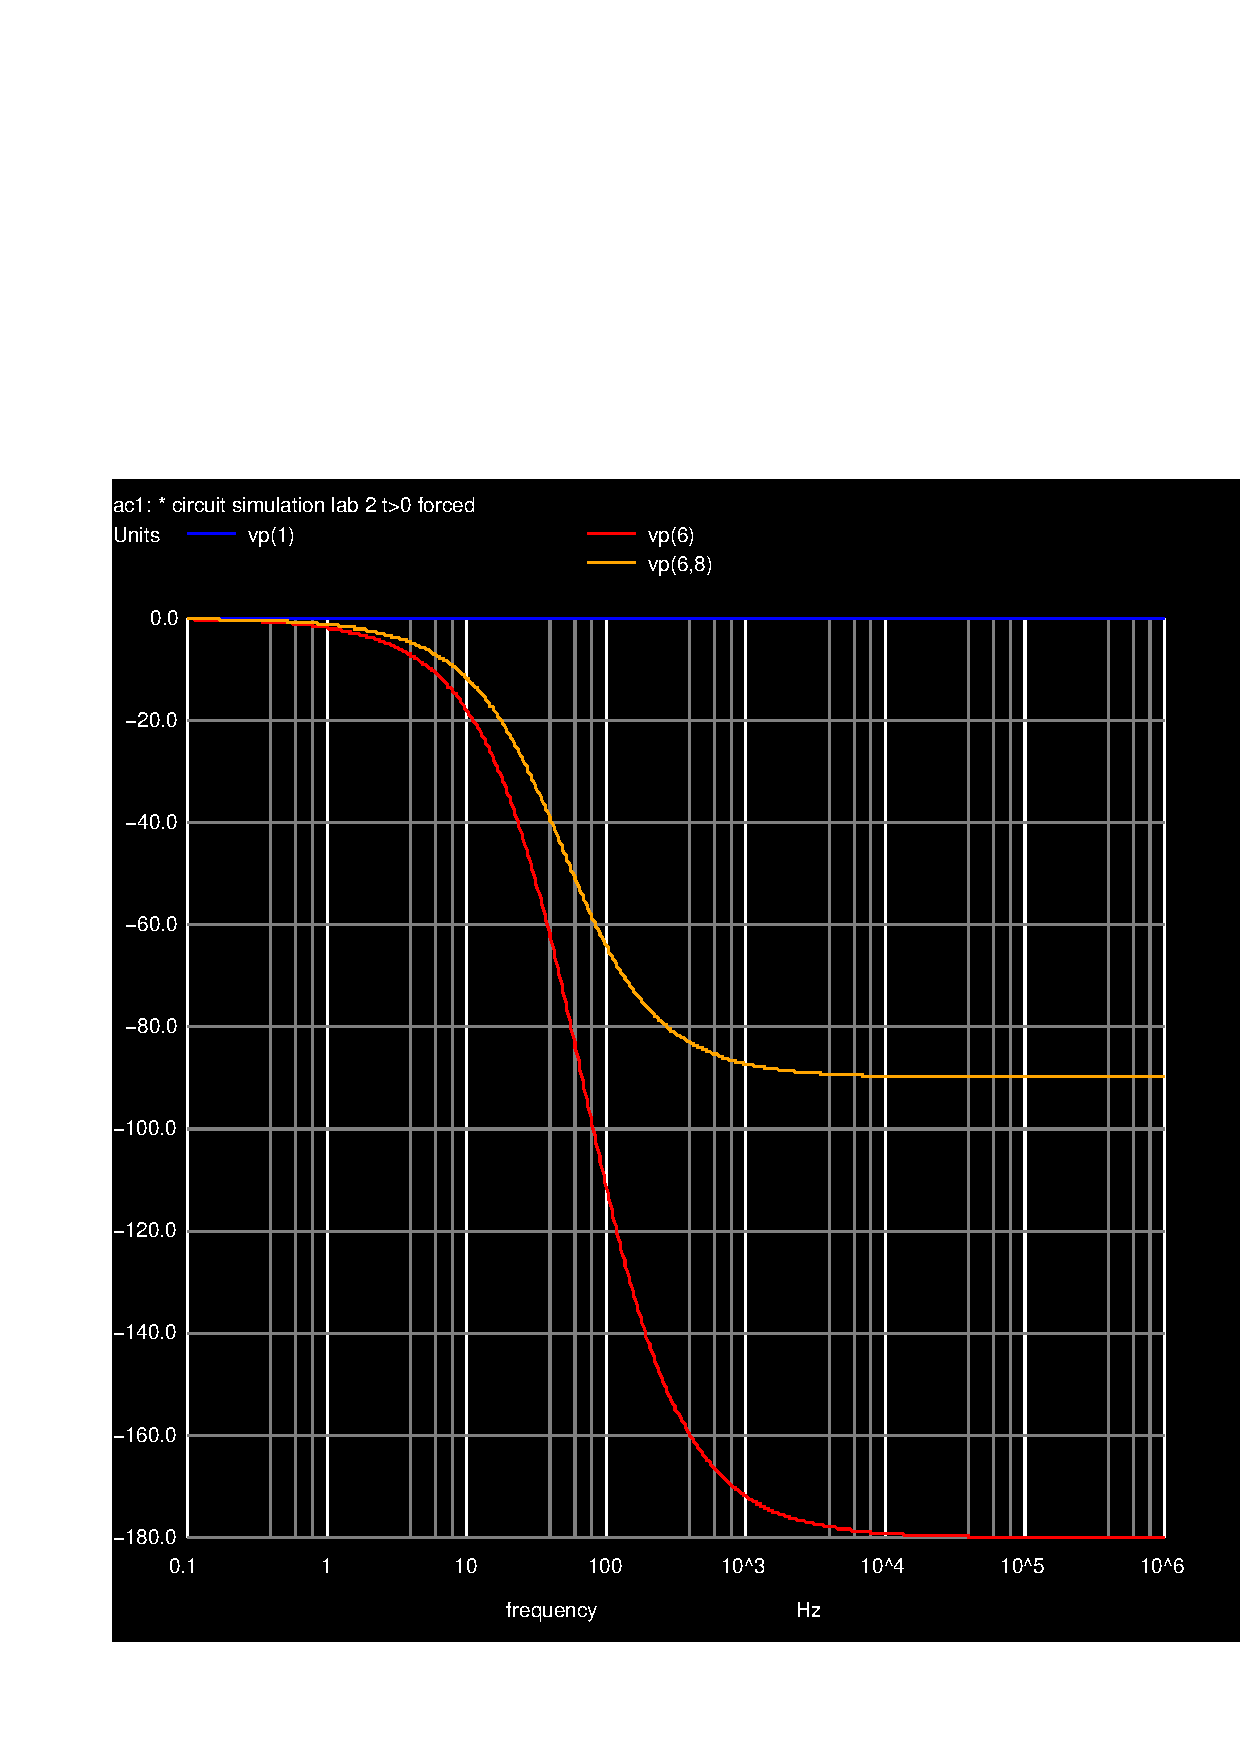
\includegraphics[width=0.4\linewidth]{../sim/phs.pdf}
\caption{Phase of V6(f), V1(f) and Vc(f) in [0,20]ms using ngspice}
\label{fig:ff}
\end{figure}
We can see these phase plots are the same, no matter the method used.
